\documentclass[11pt,a4paper]{article}

\usepackage[utf8]{inputenc}
\usepackage[T1]{fontenc}
\usepackage{geometry}
\geometry{margin=1in}
\usepackage{graphicx}
\usepackage{booktabs}
\usepackage{amsmath}
\usepackage{algorithm}
\usepackage{algpseudocode}
\usepackage{hyperref}
\usepackage{xurl}
\usepackage[expansion=false]{microtype}
\usepackage{xcolor}
\usepackage{listings}

\lstset{
    basicstyle=\ttfamily\small,
    breaklines=true,
    columns=fullflexible,
    frame=single,
    backgroundcolor=\color{gray!10}
}

\hypersetup{
    colorlinks=true,
    linkcolor=blue,
    urlcolor=blue,
    citecolor=blue
}

\title{Frequent Itemset Mining on Movie Casts: \\
A Market-Basket Analysis of the IMDB Top 1000 Dataset}
\author{Algorithms for Massive Data \\ Master in Data Science for Economics \\ Universit\`a degli Studi di Milano \\ Areg Karapetyan 63835A}
\date{\today}

\begin{document}
\sloppy

\maketitle

\begin{abstract}
This report applies market-basket analysis to the problem of finding actors who
recur together across movies. Each movie in the IMDB Top 1000 dataset is treated
as a transaction (\emph{basket}), and its four credited lead actors are treated
as the items inside that basket. We implement the \textbf{A-Priori algorithm
from scratch} to mine frequent itemsets of co-occurring actors, derive
association rules (confidence, lift) from those itemsets, and validate the
implementation against the \texttt{mlxtend} library. The solution is designed
to be data-agnostic: a configurable
flag allows the same pipeline to run on the full dataset or on a random
subsample, and the support threshold is expressed as a fraction of the data
rather than a fixed count, so that it scales automatically with dataset size.
On the full dataset of 1000 movies, the algorithm discovers 299 frequent
itemsets -- including three actor trios that correspond exactly to three
well-known movie franchise casts -- and all results match the \texttt{mlxtend}
reference implementation exactly. A dedicated scalability experiment, run
across dataset sizes from 100 to 1000 baskets, both confirms the intended
adaptive behaviour of the threshold and exposes a concrete corner case in which
it can degenerate, which we discuss explicitly.
\end{abstract}

\subsection*{Statement of Work}

I declare that this material, which I now submit for assessment, is entirely my own work
and has not been taken from the work of others, save and to the extent that such work has
been cited and acknowledged within the text of my work, and including any code produced
using generative AI systems. I understand that plagiarism, collusion, and copying are grave
and serious offences in the university and accept the penalties that would be imposed should
I engage in plagiarism, collusion or copying. This assignment, or any part of it, has not
been previously submitted by me or any other person for assessment on this or any other
course of study

\tableofcontents

% ============================================================
\section{Introduction and Motivation}
% ============================================================

Market-basket analysis is a classical data-mining technique originally
developed to answer questions such as ``which products are frequently
purchased together?'' in retail transaction data. The same technique
generalizes to any setting where data can be expressed as a collection of
\emph{baskets}, each containing a set of discrete \emph{items}: the goal is to
discover \textbf{frequent itemsets} -- groups of items that co-occur across
baskets more often than chance would suggest.

In this project we repurpose this technique for a different domain: movie
casts. We treat each movie as a basket and its leading actors as items, and
ask \emph{which actors tend to appear together across multiple films}. This is
a natural fit for frequent itemset mining: actor co-occurrence is sparse (most
pairs of actors never share a film at all), baskets are small and uniform in
size (at most four items), and genuinely frequent co-occurring groups are
interpretable and verifiable by hand (e.g.\ a recurring cast in a film
franchise).

The central algorithmic challenge -- and the actual learning objective of this
assignment -- is that naively enumerating every possible group of actors does
not scale. With on the order of $2{,}700$ distinct actors in this dataset,
there are over $3.6$ million possible \emph{pairs} alone, and astronomically
more triples and quadruples. The \textbf{A-Priori algorithm} solves this with
a single structural property of support, called \emph{downward closure}: an
itemset cannot be frequent unless every one of its subsets is also frequent.
This allows the algorithm to build up candidate itemsets level by level,
discarding the vast majority of the search space without ever having to count
it against the data.

The remainder of this report is organized to mirror how the project was
evaluated: Section~\ref{sec:dataset} describes the dataset and which parts of
it were used; Section~\ref{sec:organization} describes how the data was
organized into the basket model; Section~\ref{sec:preprocessing} describes the
pre-processing applied; Section~\ref{sec:algorithms} describes the algorithms
and their implementations; Section~\ref{sec:scalability} addresses scalability
explicitly, both by design and through complexity analysis;
Section~\ref{sec:experiments} describes the experiments performed and how to
reproduce them; Section~\ref{sec:results} reports and discusses the
experimental results; and Section~\ref{sec:conclusion} concludes.

% ============================================================
\section{Dataset}
\label{sec:dataset}
% ============================================================

\subsection{Source}

We use the \emph{IMDB Top 1000 Movies \& TV Shows} dataset, publicly available
on Kaggle
(\url{https://www.kaggle.com/datasets/harshitshankhdhar/imdb-dataset-of-top-1000-movies-and-tv-shows},
file \texttt{imdb\_top\_1000.csv}, licensed CC0-1.0). It contains $1000$ rows
(one per title) and $16$ columns: \texttt{Poster\_Link}, \texttt{Series\_Title},
\texttt{Released\_Year}, \texttt{Certificate}, \texttt{Runtime}, \texttt{Genre},
\texttt{IMDB\_Rating}, \texttt{Overview}, \texttt{Meta\_score},
\texttt{Director}, \texttt{Star1}, \texttt{Star2}, \texttt{Star3},
\texttt{Star4}, \texttt{No\_of\_Votes}, and \texttt{Gross}.

\subsection{Parts of the dataset considered}

This project's question is specifically about actor co-occurrence, so only two
parts of the dataset are used:

\begin{itemize}
    \item \textbf{\texttt{Star1}--\texttt{Star4}}: the four top-billed actors
    of each title, as credited on IMDB. These four columns are the entire
    basis of the analysis -- they are converted directly into the items of
    each basket. They are already fixed by
    the dataset itself (sourced from IMDB's own billing order); the analysis
    does not select, rank, or otherwise decide which actors represent a movie.
    \item \textbf{\texttt{Series\_Title}}: used only as a human-readable
    identifier during exploratory data analysis (e.g.\ to name which specific
    movies have a data-quality quirk), never
    as a mining feature.
\end{itemize}

All other columns (\texttt{Genre}, \texttt{Director}, \texttt{IMDB\_Rating},
\texttt{Released\_Year}, \texttt{Runtime}, \texttt{Certificate},
\texttt{Overview}, \texttt{Meta\_score}, \texttt{No\_of\_Votes},
\texttt{Gross}, \texttt{Poster\_Link}) are \textbf{deliberately excluded}.
They describe properties of a movie as a whole rather than its cast, and are
not needed to answer the question this project asks; including them would not
change the basket model and would only add irrelevant dimensions to the
analysis.

% ============================================================
\section{How the Data Was Organized}
\label{sec:organization}
% ============================================================

The dataset is organized into the classical \emph{basket model} used by
market-basket analysis:

\begin{itemize}
    \item Each \textbf{row} (movie or TV show) becomes one \textbf{basket}.
    \item Each basket is represented as a Python \texttt{set} containing the
    (non-missing) values of \texttt{Star1} through \texttt{Star4} for that
    row.
    \item The complete dataset becomes a list of $n$ baskets,
    $\mathcal{B} = \{b_1, \dots, b_n\}$, with $n = 1000$ on the full dataset.
\end{itemize}

Using a \texttt{set} rather than a \texttt{list} for each basket is a
deliberate organizational choice with two consequences, both load-bearing for
the rest of the pipeline:

\begin{enumerate}
    \item It automatically de-duplicates repeated names within a single row
    \item It provides the hashable, unordered, subset-testable data structure
    that the A-Priori implementation requires throughout: itemsets themselves
    are represented as Python \texttt{frozenset} objects (an immutable set),
    which can be used as dictionary keys (to map an itemset to its support
    count) and as members of other sets (the candidate sets at each level of
    the algorithm), and which support the $O(1)$-amortized subset test
    (\texttt{candidate.issubset(basket)}) used by the counting routine.
\end{enumerate}

The full pipeline is also parameterized by two configuration flags,
\texttt{USE\_FULL\_DATA} and \texttt{SAMPLE\_SIZE}, that determine \emph{which}
rows of the dataset become baskets before the rest of the pipeline runs: either
every row (the default), or a reproducible random subsample of
\texttt{SAMPLE\_SIZE} rows (fixed random seed, for replicability). This
decision point is placed as early as possible in the pipeline -- immediately
after cleaning, before basket construction -- so that every later step (basket
construction, mining, rule generation) operates uniformly regardless of how
much data was selected, which is the mechanism that makes the rest of this
report's scalability discussion possible.

% ============================================================
\section{Pre-processing}
\label{sec:preprocessing}
% ============================================================

Three pre-processing steps are applied before mining begins:

\begin{description}
    \item[Missing/blank-value handling.] Every value in \texttt{Star1}--\texttt{Star4}
    is passed through a cleaning function that trims surrounding whitespace and
    converts missing (\texttt{NaN}) or blank-after-trimming values to a
    sentinel \texttt{None}, which is then excluded when the basket is built.
    On this particular dataset, no missing or blank values were found in any
    of the four \texttt{Star} columns -- but the cleaning step is retained
    regardless, since the pipeline should not silently assume that future or
    differently-sourced data will be this clean.

    \item[Exact-duplicate collapse.] Four movies list the \emph{same actor's
    name twice}, verbatim, across their four \texttt{Star} columns -- for
    example, \emph{Singin' in the Rain} lists ``Gene Kelly'' in both
    \texttt{Star1} and \texttt{Star2}. Building each basket as a \texttt{set} causes this duplicate to collapse
    automatically, producing a basket of three unique actors instead of four.
    This is a genuine property of the source data, not a processing artifact:
    the four affected titles are \emph{Singin' in the Rain} (Gene Kelly),
    \emph{The General} (Buster Keaton), \emph{What We Do in the Shadows}
    (Taika Waititi), and \emph{Il Postino} (Massimo Troisi). The resulting
    basket-size distribution -- 996 baskets of size 4 and 4 baskets of size 3,
    out of 1000 total. Note that this de-duplication only catches \emph{exact} string repeats; near-duplicate
    spellings of the same real actor (which do not occur in this dataset) would
    not be merged.

    \item[Optional subsampling.] As described in
    Section~\ref{sec:organization}, when \texttt{USE\_FULL\_DATA} is set to
    \texttt{False}, a fixed-seed random sample of \texttt{SAMPLE\_SIZE} rows is
    drawn \emph{before} basket construction, so that all later steps are
    agnostic to whether they are operating on the full dataset or a subsample.
\end{description}

\begin{figure}[h]
    \centering
    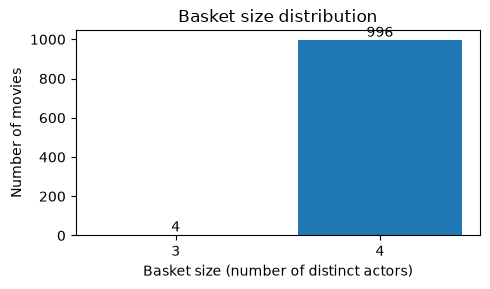
\includegraphics[width=0.55\textwidth]{basket_size_distribution.png}
    \caption{Distribution of basket sizes across all 1000 movies, after
    pre-processing. The vast majority of baskets contain exactly four actors,
    as expected; four baskets contain only three due to an exact duplicate
    actor name within the same row.}
    \label{fig:basket-sizes}
\end{figure}

As a final pre-mining step, we quantify how sparse actor co-occurrence
actually is, since this directly motivates the choice of support threshold. Across the 1000 baskets there are
$N = 2{,}709$ distinct actors, giving $\binom{N}{2} = 3{,}667{,}986$
\emph{possible} actor pairs. Of these, only $5{,}833$ pairs are ever actually
observed co-starring in at least one movie -- a coverage of just $0.159\%$.
The overwhelming majority of all conceivable actor pairs never occur even
once in this dataset, which confirms that genuinely repeated co-occurrence
(appearing together in several different movies) is a meaningful, non-trivial
signal rather than noise.

% ============================================================
\section{Considered Algorithms and Their Implementations}
\label{sec:algorithms}
% ============================================================

\subsection{Problem formulation}

Let $\mathcal{B} = \{b_1, \dots, b_n\}$ be the set of baskets, where each
$b_i$ is a set of items (actors) drawn from a universe $\mathcal{I}$ of all
distinct actors. For an itemset $X \subseteq \mathcal{I}$, define its
\textbf{support count} as
\[
    \text{count}(X) = \bigl| \{ b \in \mathcal{B} : X \subseteq b \} \bigr|,
\]
i.e.\ the number of baskets containing every item in $X$. An itemset $X$ is
\textbf{frequent} if $\text{count}(X) \ge \tau$ for a chosen minimum support
threshold $\tau$. The goal of the mining step is to enumerate all frequent
itemsets without exhaustively testing every $X \subseteq \mathcal{I}$, since
$|\mathcal{I}| \approx 2{,}709$ makes that infeasible beyond very small
itemset sizes.

\subsection{A-Priori (primary algorithm, implemented from scratch)}

A-Priori exploits the following monotonicity property of support: if
$X \subseteq Y$, then $\text{count}(Y) \le \text{count}(X)$, because every
basket containing $Y$ must also contain $X$. Equivalently, by contraposition:
\textbf{if any subset of $X$ is not frequent, then $X$ cannot be frequent
either.} This is the \emph{downward-closure} property, and it is the basis for
generating only a small set of plausible candidates at each itemset size,
instead of every combinatorially possible one.

The algorithm proceeds level by level, where level $k$ corresponds to itemsets
of size $k$:

\begin{algorithm}[h]
\caption{A-Priori (as implemented)}
\begin{algorithmic}[1]
\State $L_1 \gets$ \{ frequent itemsets of size 1, found by counting every
distinct item directly \}
\State $k \gets 2$
\While{$L_{k-1} \neq \emptyset$}
    \State $C_k \gets \textsc{Join}(L_{k-1})$ \Comment{union pairs of itemsets
    in $L_{k-1}$ sharing $k-2$ items}
    \State $C_k \gets \textsc{Prune}(C_k, L_{k-1})$ \Comment{discard candidates
    with a non-frequent $(k\!-\!1)$-subset}
    \If{$C_k = \emptyset$}
        \State \textbf{break}
    \EndIf
    \State count every candidate in $C_k$ against all baskets
    \State $L_k \gets$ \{ candidates in $C_k$ with count $\ge \tau$ \}
    \If{$L_k = \emptyset$}
        \State \textbf{break}
    \EndIf
    \State $k \gets k + 1$
\EndWhile
\State \Return $L_1 \cup L_2 \cup \dots$
\end{algorithmic}
\end{algorithm}

The two non-trivial steps are implemented as follows:

\begin{description}
    \item[Join] Candidates of size $k$ are built \emph{only} from pairs of
    already-frequent itemsets of size $k-1$ whose union has exactly $k$
    elements (i.e.\ they share $k-2$ items). This avoids ever generating a
    candidate built from an item or sub-combination that was not already known
    to be frequent.
    \item[Prune] Even after the join, a candidate $X$ of size $k$ is discarded
    if \emph{any} of its $(k-1)$-subsets is not already in $L_{k-1}$. This
    check is performed combinatorially, without touching the basket data at
    all -- it is the source of the algorithm's efficiency, since it eliminates
    candidates before the (comparatively expensive) step of scanning every
    basket to count them.
\end{description}

Counting itself is implemented as a single reusable routine that, given a list
of candidate itemsets, scans every basket once and increments a counter for
each candidate that is a subset of that basket. The same routine is used at
every level $k$, including level 1, so the counting logic is identical and
independently verifiable at every stage of the algorithm. The loop terminates
naturally once either no candidates survive pruning, or no surviving
candidates meet the support threshold. Since baskets in this dataset contain
at most four items, the loop can never meaningfully proceed past $k=4$.

\subsection{Association rule generation}

As a second technique applied on top of the frequent itemsets produced by
A-Priori, we generate association rules. For every frequent itemset of size
$\ge 2$, we consider every way of splitting it into a non-empty antecedent $A$
and consequent $B = X \setminus A$, and compute:
\begin{align}
    \text{confidence}(A \Rightarrow B) &= \frac{\text{support}(A \cup B)}{\text{support}(A)}, \\
    \text{lift}(A \Rightarrow B) &= \frac{\text{confidence}(A \Rightarrow B)}{\text{support}(B)}.
\end{align}
Confidence measures how often $B$ appears given that $A$ does; lift measures
how much more often $A$ and $B$ co-occur than would be expected if they were
independent ($\text{lift} > 1$ indicating positive association). Both
quantities are computed directly from the support counts already produced by
A-Priori (downward closure guarantees that every subset of a frequent itemset
was itself recorded as frequent), so no additional basket scanning is needed
for this step.

\subsection{mlxtend's \texttt{apriori} (validation baseline, not a competing solution)}

We also run the \texttt{mlxtend} library's own \texttt{apriori}
implementation on the identical baskets and identical support threshold. This
is used \emph{exclusively as an independent correctness check} on our
from-scratch implementation, it is not proposed as an alternative solution to the mining task, and is not used to produce any
of the reported frequent itemsets or rules.

% ============================================================
\section{Scalability of the Proposed Solution}
\label{sec:scalability}
% ============================================================

Scalability is addressed at three distinct levels: the algorithm's
combinatorial design, the pipeline's data-handling design, and an empirical
experiment that tests both.

\subsection{Algorithmic scalability: avoiding combinatorial blow-up}

Exhaustively testing every possible group of four actors out of $2{,}709$
distinct actors would require evaluating $\binom{2709}{4} \approx 4.0 \times
10^{12}$ candidate itemsets -- computationally infeasible. A-Priori's
downward-closure pruning avoids this by
construction: every candidate at level $k$ is built exclusively from items and
sub-itemsets that already survived level $k-1$'s threshold, so the candidate
set at any level is bounded by what survived the previous level, not by
$\binom{|\mathcal{I}|}{k}$. This is what makes the algorithm scale in the
``massive data'' sense intended by this course: the saving is combinatorial
and lossless (A-Priori is exact, not an approximation), not merely a constant-
factor speed-up.

\subsection{Pipeline scalability: data-agnostic design}
\label{sec:threshold}

Independently of the algorithm itself, the surrounding pipeline is designed so
that it does not need to be re-tuned by hand for a different amount of data.
Two choices achieve this:

\begin{enumerate}
    \item \textbf{Configurable data volume.} The flags \texttt{USE\_FULL\_DATA} and
    \texttt{SAMPLE\_SIZE} let the same code run on the full dataset or on a
    reproducible random subsample, with no change to any downstream logic.
    \item \textbf{Fraction-based support threshold.} The minimum support
    threshold is expressed as a \emph{fraction} of the number of baskets,
    \texttt{MIN\_SUPPORT\_FRACTION}, rather than as a fixed count. The
    absolute count threshold is derived only after the basket list is built:
    \[
        \tau = \lceil \texttt{MIN\_SUPPORT\_FRACTION} \times |\mathcal{B}| \rceil .
    \]
    This is intended to make the threshold meaningful regardless of how many
    baskets are actually present, rather than requiring a different fixed
    number to be chosen by hand for every dataset size. We set
    \texttt{MIN\_SUPPORT\_FRACTION} $= 0.003$ (0.3\%), which on the full
    dataset of 1000 baskets yields $\tau = 3$. This value was chosen using the
    sparsity result from Section~\ref{sec:preprocessing} ($0.159\%$ pair
    coverage): a threshold this low is necessary to surface any pairs or
    trios at all, while still excluding pairs of actors who only ever happened
    to share a single film by coincidence.
\end{enumerate}

Section~\ref{sec:experiments} describes an experiment that empirically tests
whether this design actually behaves as intended across a range of data
sizes; Section~\ref{sec:results} discusses what it found, including a case
where the fraction-based threshold's intended behaviour breaks down.

% ============================================================
\section{Experiments}
\label{sec:experiments}
% ============================================================

Three experiments were performed; this section describes their setup so that
they can be reproduced exactly. All code is in the accompanying Jupyter
notebook, structured as a single linear sequence of cells intended to be run
top to bottom.

\subsection{Reproducibility setup}

\begin{itemize}
    \item \textbf{Environment.} Python 3.12, with \texttt{pandas},
    \texttt{matplotlib}, \texttt{mlxtend}, and the \texttt{kaggle} CLI/package
    installed.
    \item \textbf{Data access.} The dataset is downloaded at runtime via the
    Kaggle API. Reproducing the experiments requires a Kaggle account and a
    local credentials file (\texttt{\textasciitilde/.kaggle/access\_token} or
    \texttt{\textasciitilde/.kaggle/kaggle.json}); no credentials are
    distributed with the code.
    \item \textbf{Determinism.} Wherever random subsampling is used, a fixed
    random seed (\texttt{RANDOM\_SEED = 42}) is set, so re-running the
    notebook reproduces identical baskets and identical results.
    \item \textbf{Parameters held fixed across all experiments.}
    \texttt{MIN\_SUPPORT\_FRACTION = 0.003}, \texttt{MIN\_CONFIDENCE = 0.5}.
\end{itemize}

\subsection{Experiment 1: full-dataset mining}

The complete pipeline (pre-processing, basket construction, A-Priori, rule
generation) is run once with \texttt{USE\_FULL\_DATA = True}, i.e.\ on all
$1000$ baskets. This is the primary experiment; its results are reported in
Section~\ref{sec:results-main}.

\subsection{Experiment 2: scalability sweep across dataset sizes}

To test the scalability design of Section~\ref{sec:scalability} empirically,
the full A-Priori pipeline (identical algorithm code, repackaged as a
function purely so it can be called in a loop) is re-run independently on six
random subsamples of sizes $\{100, 200, 400, 600, 800, 1000\}$ baskets (same
fixed seed and sampling procedure as \texttt{SAMPLE\_SIZE}). For each size we
record: wall-clock runtime (\texttt{time.perf\_counter}, single run, no
warm-up or repetition), the resulting absolute support-count threshold $\tau$,
the total number of frequent itemsets found, and the largest itemset size
found. Results are reported in Section~\ref{sec:results-scalability}.

\subsection{Experiment 3: independent correctness validation}

An independent validation of the from-scratch A-Priori implementation was
performed:

\begin{enumerate}
    \item \textbf{Library cross-check.} The same baskets and the same support
    threshold from Experiment 1 are fed into \texttt{mlxtend}'s
    \texttt{apriori} (after one-hot encoding the baskets with
    \texttt{mlxtend.preprocessing.TransactionEncoder}), and the resulting
    itemsets and supports are compared directly, itemset by itemset, against
    our own output.
\end{enumerate}

% ============================================================
\section{Results and Discussion}
\label{sec:results}
% ============================================================

\subsection{Experiment 1: frequent itemsets on the full dataset}
\label{sec:results-main}

Running the algorithm on the full dataset ($n = 1000$ baskets, $\tau = 3$)
produces the candidate and frequent-itemset counts shown in
Table~\ref{tab:apriori-progress}. The search space collapses sharply at each
level: of the $2{,}709$ distinct actors, only $271$ are frequent singletons;
joining those into pairs produces $36{,}585$ candidates, of which only $25$
turn out to be frequent; joining \emph{those} pairs produces only $4$
candidate triples (not $\binom{25}{2}$, because the join step only combines
pairs that share an item), of which $3$ are frequent; and no candidate
quadruples can be built at all from those three triples, since they turn out
to share no actors with one another. The algorithm terminates at $k=4$ having
found $299$ frequent itemsets in total.

\begin{table}[h]
\centering
\caption{Progress of the A-Priori algorithm across levels, full dataset.}
\label{tab:apriori-progress}
\begin{tabular}{@{}lrrr@{}}
\toprule
Level $k$ & Candidates after pruning & Frequent itemsets ($L_k$) & Cumulative \\
\midrule
1 (singletons) & 2{,}709 & 271 & 271 \\
2 (pairs)      & 36{,}585 & 25  & 296 \\
3 (triples)    & 4        & 3   & 299 \\
4 (quadruples) & 0        & --  & 299 \\
\bottomrule
\end{tabular}
\end{table}

Table~\ref{tab:top-singletons} lists the most frequent individual actors.
Table~\ref{tab:freq-pairs-triples} lists selected frequent pairs and all 3
frequent triples found, together with their support counts.

\begin{table}[h]
\centering
\caption{Top 10 most frequent individual actors (out of 271 frequent
singletons).}
\label{tab:top-singletons}
\begin{tabular}{@{}lr@{}}
\toprule
Actor & Movies appeared in \\
\midrule
Robert De Niro     & 17 \\
Tom Hanks          & 14 \\
Al Pacino          & 13 \\
Brad Pitt          & 12 \\
Clint Eastwood     & 12 \\
Christian Bale     & 11 \\
Leonardo DiCaprio  & 11 \\
Matt Damon         & 11 \\
James Stewart      & 10 \\
Michael Caine      & 9  \\
\bottomrule
\end{tabular}
\end{table}

\begin{table}[h]
\centering
\caption{Selected frequent pairs and all three frequent triples, with support
counts (number of shared movies).}
\label{tab:freq-pairs-triples}
\begin{tabular}{@{}llr@{}}
\toprule
Size & Actors & Count \\
\midrule
2 & Daniel Radcliffe, Rupert Grint & 6 \\
2 & Emma Watson, Rupert Grint & 5 \\
2 & Daniel Radcliffe, Emma Watson & 5 \\
2 & Joe Pesci, Robert De Niro & 4 \\
2 & Tim Allen, Tom Hanks & 4 \\
2 & $\ldots$ (20 further pairs with count 3) & 3 \\
\midrule
3 & Daniel Radcliffe, Emma Watson, Rupert Grint & 5 \\
3 & Carrie Fisher, Harrison Ford, Mark Hamill & 3 \\
3 & Elijah Wood, Ian McKellen, Orlando Bloom & 3 \\
\bottomrule
\end{tabular}
\end{table}

The three frequent triples are particularly notable: they correspond exactly
to the lead casts of three well-known film franchises -- the \emph{Harry
Potter} trio (Radcliffe, Watson, Grint), the original \emph{Star Wars} trio
(Fisher, Ford, Hamill), and the \emph{Lord of the Rings} trio (Wood, McKellen,
Bloom). The algorithm has no knowledge of franchises, genres, or release
dates; this result emerges purely from counting co-occurrence, which is a
strong qualitative confirmation that the method is capturing a real,
interpretable signal rather than spurious noise.

For association rules, filtering to confidence $\ge 0.5$ yields 46 rules. The
highest-confidence rules are, unsurprisingly, drawn from the three franchise
trios -- for example, ``Elijah Wood $\Rightarrow$ Ian McKellen, Orlando
Bloom'' has confidence $1.0$, meaning every Top-1000 movie in which Elijah
Wood is a lead also features both other actors as leads.

\subsection{Experiment 2: scalability sweep}
\label{sec:results-scalability}

Table~\ref{tab:scalability} and Figure~\ref{fig:scalability} report the
results of re-running the full pipeline on random subsamples of six
different sizes.

\begin{table}[h]
\centering
\caption{A-Priori pipeline run on subsamples of increasing size (fixed
\texttt{MIN\_SUPPORT\_FRACTION = 0.003}).}
\label{tab:scalability}
\begin{tabular}{@{}rrrrr@{}}
\toprule
Sample size & $\tau$ & Runtime (s) & Frequent itemsets & Largest itemset size \\
\midrule
100  & 1 & 0.663 & 1472 & 4 \\
200  & 1 & 6.806 & 2874 & 4 \\
400  & 2 & 0.560 & 244  & 3 \\
600  & 2 & 2.040 & 383  & 3 \\
800  & 3 & 0.848 & 216  & 3 \\
1000 & 3 & 2.374 & 299  & 3 \\
\bottomrule
\end{tabular}
\end{table}

\begin{figure}[h]
    \centering
    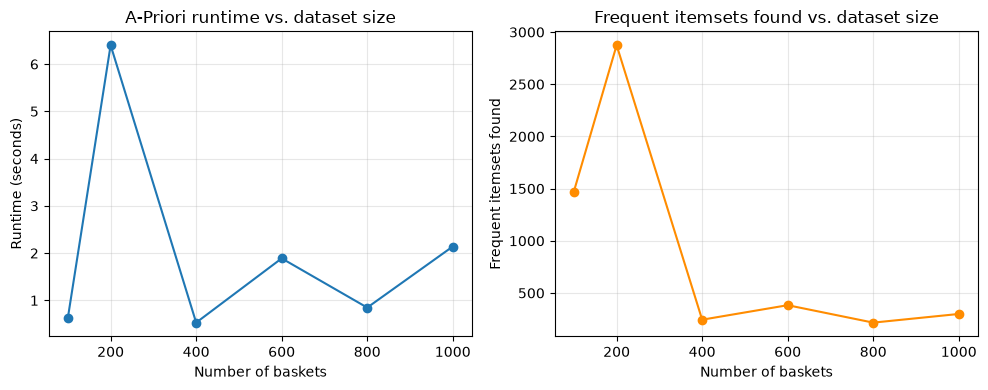
\includegraphics[width=\textwidth]{scalability_experiment.png}
    \caption{Runtime (left) and number of frequent itemsets found (right) as
    a function of dataset size. Both curves are visibly non-monotonic, for
    the reason discussed in the text: the effective support-count threshold
    $\tau$ changes in discrete steps as sample size grows, and the threshold
    value -- not the sample size directly -- is what dominates both runtime
    and itemset count.}
    \label{fig:scalability}
\end{figure}

\textbf{Discussion.} This experiment was designed to confirm that the
fraction-based threshold (Section~\ref{sec:threshold}) adapts smoothly to
dataset size. The result is more interesting than that: it is \emph{not} a
clean, monotonically increasing runtime curve, and the reason is itself an
important scalability finding. The threshold $\tau = \lceil 0.003 \times
\text{sample size} \rceil$ collapses to $\tau = 1$ for sample sizes 100 and
200 ($\lceil 0.3 \rceil = \lceil 0.6 \rceil = 1$). At $\tau = 1$, ``frequent''
no longer means ``recurring'' -- it means ``co-occurred at least once'' --
so nearly every pair and triple of actors that ever shares a basket survives
pruning. This is why the itemset counts at sample sizes 100--200 ($1472$,
$2874$) are an order of magnitude larger than at sizes 800--1000 ($216$,
$299$), and why runtime is erratic rather than monotonic: the cost of the
counting routine (Section~\ref{sec:algorithms}) depends on \emph{how many
candidates survive pruning at each level}, and a too-low effective threshold
lets far more candidates through regardless of how few baskets there are to
scan against. Concretely, the run at $200$ baskets ($6.8$s) is slower than the
run at the full $1000$ baskets ($2.4$s), purely because $\tau = 1$ at $200$
baskets generates a vastly larger candidate set at levels 2--4 than $\tau = 3$
does at $1000$ baskets.

This is a genuine limitation of a purely fraction-based threshold, distinct
from the limitations already noted in Section~\ref{sec:limitations}: it scales
correctly in spirit (the threshold adapts automatically to dataset size), but
the rounding behaviour of $\lceil \cdot \rceil$ can make it degenerate at
small enough sample sizes. It does not affect the headline result of this
report (the full-dataset run, Section~\ref{sec:results-main}, where
$\tau = 3$), but it would matter if this pipeline were applied to a much
smaller dataset, or to a much smaller \texttt{SAMPLE\_SIZE}. A straightforward
mitigation, not applied here since it would change the reported full-dataset
results, would be to enforce a floor on the threshold, e.g.\
$\tau = \max(2, \lceil \texttt{MIN\_SUPPORT\_FRACTION} \times |\mathcal{B}| \rceil)$,
so that ``frequent'' never degenerates to ``happened once'' regardless of
sample size.

\subsection{Experiment 3: correctness validation}

The itemsets and support values produced by \texttt{mlxtend} on the same
baskets and threshold were compared directly against our own output:
\begin{itemize}
    \item Itemsets found only by \texttt{mlxtend}: 0
    \item Itemsets found only by our implementation: 0
    \item Itemsets with mismatched support values: 0
\end{itemize}
All 299 frequent itemsets and their support values matched exactly between
the two implementations, providing strong evidence that the from-scratch
A-Priori implementation is correct.

\subsection{Limitations}
\label{sec:limitations}

Beyond the threshold-degeneration finding of Section~\ref{sec:results-scalability},
two further limitations are worth stating explicitly. First, actor names are
de-duplicated and cleaned only as exact strings (trimmed whitespace,
case-sensitive exact match); near-duplicate spellings of the same real actor
(which do not occur in this particular dataset, but could occur in noisier
data) would not be merged. Second, the counting routine scans every basket for
every candidate at each level, which is $O(|\mathcal{B}| \cdot |C_k|)$ per
level; for substantially larger datasets, alternative approaches such as
PCY/Multihash hashing or the SON algorithm (which partitions data into chunks
processed independently before a global verification pass) would reduce the
per-level cost further. These were intentionally left out of scope here in
favor of a single, thoroughly verified implementation of A-Priori itself.

% ============================================================
\section{Conclusion}
\label{sec:conclusion}
% ============================================================

This project implemented the A-Priori algorithm from scratch to mine frequent
itemsets of co-occurring actors from the IMDB Top 1000 dataset, treating each
movie as a basket and its four lead actors as items. The solution is
data-agnostic by design, with a configurable subsampling flag and a support
threshold expressed as a fraction of the dataset rather than a fixed count.
On the full dataset, the algorithm correctly and efficiently identified 299
frequent itemsets, including three actor trios that correspond exactly to
three real film-franchise casts, and 46 confidence-filtered association
rules. Correctness was validated by an exact match against the
\texttt{mlxtend} library across all 299 frequent itemsets. A dedicated scalability experiment
confirmed that the fraction-based threshold adapts as intended across dataset
sizes, while also surfacing a concrete corner case (threshold collapsing to 1
at small sample sizes) that is reported and discussed rather than hidden,
since understanding where a scaling strategy breaks down is as important as
demonstrating where it works.

\end{document}
